\documentclass[11pt,a4paper]{article}

%---------------------------------------------------------
%	Aditional Packages
%--------------------------------------------------------
\usepackage{textpos}
\usepackage{subcaption} % To have multiple plots side by side
\usepackage{float}
\usepackage{url} % enable clickable URLs
\usepackage{listings} % to have code blocks in your document
\usepackage{xcolor}
\usepackage{doi}
\usepackage{microtype}
\usepackage{booktabs}
\usepackage{nicefrac} % creates a fraction that is nicer when used in text \nicefrac{1}{2}

% Define some colors for code 
\definecolor{codegreen}{rgb}{0,0.6,0}
\definecolor{codegray}{rgb}{0.5,0.5,0.5}
\definecolor{codepurple}{rgb}{0.58,0,0.82}
\definecolor{backcolour}{rgb}{0.95,0.95,0.92}

% Defines codeblock styles
\lstdefinestyle{mystyle}{
    backgroundcolor=\color{backcolour},   
    commentstyle=\color{codegreen},
    keywordstyle=\color{magenta},
    numberstyle=\tiny\color{codegray},
    stringstyle=\color{codepurple},
    basicstyle=\ttfamily\footnotesize,
    breakatwhitespace=false,         
    breaklines=true,                 
    captionpos=b,                    
    keepspaces=true,                 
    numbers=left,                    
    numbersep=5pt,                  
    showspaces=false,                
    showstringspaces=false,
    showtabs=false,                  
    tabsize=2
}

% Set the maximum depth sections are counted to and shown in the TOC
\setcounter{secnumdepth}{3} % depth of counting
\setcounter{tocdepth}{3} % depth that toc will show 

% new paragraph style with new line
\newcommand{\myparagraph}[1]{\paragraph{#1}\mbox{}\\}


\lstset{style=mystyle}
\renewcommand{\lstlistingname}{Configuration}% Listing -> Configuration

% Toogle between the two to hide or show images
% \usepackage[draft]{graphicx}
\usepackage{graphicx}
\usepackage[utf8]{inputenc} 
\usepackage{upgreek}
\usepackage{titlesec}
\usepackage{physics} % adds easy derivatives etc. 
%\AtBeginDocument{\RenewCommandCopy\qty\SI} % dont know why
\usepackage{amssymb} % more symbols
\usepackage{amsmath} %enables align environment
\usepackage{multirow}


% \usepackage[showframe]{geometry} % Shows margins in pdf if you want to know what's going on
\usepackage{geometry}
\geometry{
    %a4paper,
	left=40mm,
    % right=20mm,
	top=35mm,
    }

% Use biblatex
\usepackage[backend=biber,
natbib=true,
maxcitenames = 2,
maxbibnames = 5,
minbibnames = 4, 
sorting=none]{biblatex}

\usepackage{csquotes}

\addbibresource{references.bib}
\setlength\bibitemsep{1.5\itemsep}


% --------------------------------------------------------
% CUSTOM STUFF:
\usepackage[textsize=tiny]{todonotes}
\setlength{\marginparwidth}{2cm}
\usepackage{bm}
\usepackage{tikz}
\newcommand{\no}{%
\tikz[scale=0.23] {
    \draw[line width=0.7,line cap=round] (0,0) to [bend left=6] (1,1);
    \draw[line width=0.7,line cap=round] (0.2,0.95) to [bend right=3] (0.8,0.05);
}}
\newcommand{\yes}{%
\tikz[scale=0.23] {
    \draw[line width=0.7,line cap=round] (0.25,0) to [bend left=10] (1,1);
    \draw[line width=0.8,line cap=round] (0,0.35) to [bend right=1] (0.23,0);
}}
\usepackage[table]{xcolor}
%---------------------------------------------------------
\usepackage{hyperref} % enable clickable links to sections, figures, etc. 
\PassOptionsToPackage{unicode}{hyperref}
\PassOptionsToPackage{naturalnames}{hyperref}

% Remove the coloured border around autoref links
\hypersetup{%
pdfborder = {0 0 0}
}



\begin{document}	
\pagestyle{empty}

%---------------------------------------------------------
%	Titlepage
%---------------------------------------------------------

\begin{center}
    \vspace*{1cm}
    \LARGE \bf{Structure recognition with graph neural networks} \\

    \vspace*{2cm}
    \large \bf{A report for the course "Advanced Projects in Computational Physics 2"}


    \vspace{4cm}
    
    \vspace{1.2cm}
            From\\
            {\bf Stephen Weybrecht} \\
            \today

    \vspace*{6 cm}
    Supervisor: Jonas Buba 
    \vspace*{1 cm}

\end{center}
\clearpage

\begin{abstract}
The project described in the following lies at the intersection of solid-state physics and machine learning. On the one hand, there is a physical problem regarding crystal lattices in 2 and 3 dimensions, namely their classification into Bravais lattice groups and defect detection. For an efficient and robust classification regardless of noise and introduced defects, neural networks promise an interesting approach and will therefore be the second part of this project. Special networks designed for handling graph-like structures, so-called graph convolutional networks are employed. These use a concept called message passing to efficiently enable classification tasks. \\

The basics behind Bravais lattices, Machine Learning and graph neural networks are discussed in \autoref{sec:Theoretical introduction}. 
In \autoref{sec:Results} these networks are first used for a graph-level classification task in order to gain familiarity with the architecture. After this an advanced application is discussed: building a graph autoencoder for outlier detection. While for the first task test accuracies of around 94\% (2D) and 87\% (3D) have been reached the second task has proven itself to be challenging. Different tests are therefore performed, analyzed and discussed. 
In \autoref{sec:Conclusion} a conclusion is drawn, summarizing the achievements of the project and ideas for further investigations. 
\end{abstract}

\clearpage
\tableofcontents
\restoregeometry
\clearpage
\mbox{}

\pagenumbering{arabic}
\setcounter{page}{1}
\pagestyle{plain}
%---------------------------------------------------------
%   Report
%---------------------------------------------------------

\section{Theoretical introduction}
\label{sec:Theoretical introduction}

\subsection{Bravais lattices}
\label{ssec:Bravais lattices}
In the first part of the project, our task was to deal with crystal lattices in 2 and 3 dimensions. 
For the following discussion an introduction of the terms "crystal", "basis" and "Bravais lattice" is therefore needed. \\

Following the discussion of \cite{kittelChapter1Crystal2005} an ideal crystal is a periodic, infinite arrangement of atoms in a solid. 
These atoms are arranged in blocks, a so-called basis, in a regularly spaced grid, the lattice. 
In other words, the lattice represents a schema after which individual atoms or groups of atoms (the basis) are arranged to form the crystal. 
A lattice in $d$ dimensions can be defined by a set of $d$ translation vectors. 
The superposition of integer multiples of these vectors then makes up the lattice \cite{kittelChapter1Crystal2005}. 
In principle, the length and direction of these vectors can be arbitrary. 
In this case, the lattice would generally not map into itself under translations and rotations -- it is called oblique. 
There are however special sets of translation vectors that form lattices of high symmetry. 
These fundamental lattices are called the Bravais lattices. 
For $d=2$ there are 5 (4 special and one oblique) Bravais lattices, while for $d=3$ there are 14 (13 special cases and one oblique, so-called triclinic lattice). 
These are depicted in \autoref{fig:bravais2D} and \autoref{fig:bravais3D} respectively. 

\begin{figure}[htbp]
\centering
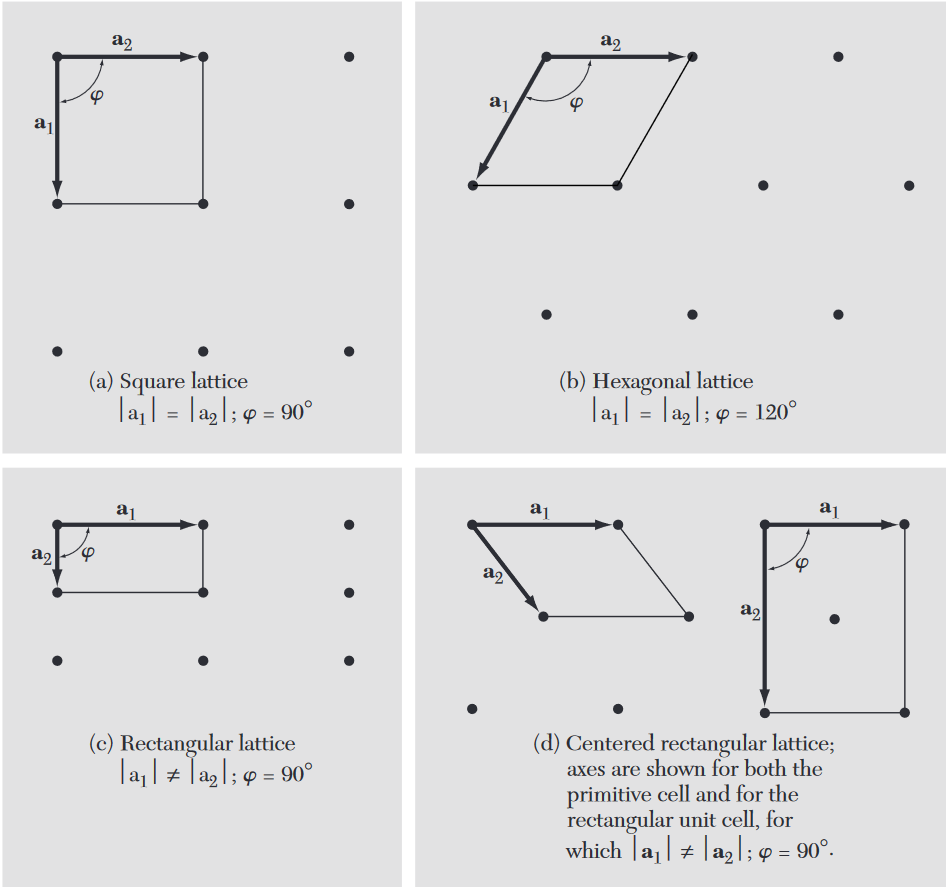
\includegraphics[width=0.6\textwidth]{images/Kittel_7.png}
\caption{The five Bravais lattices for 2 dimensions. The graphic also illustrates the length of the translation vectors $\bm{a}_i$ and the angle between them to make up the corresponding lattice. Taken from \cite[Fig. 7]{kittelChapter1Crystal2005}.}
\label{fig:bravais2D}
\end{figure}

\begin{figure}[htbp]
\centering
\includegraphics[width=0.7\textwidth]{images/Kittel_14.png}
\caption{The 14 Bravais lattices for the $d=3$ case. 
One further classifies these lattices into seven types of cells: Cubic ($a{=}b{=}c$, $\alpha {=} \beta {=} \gamma{=}90^\circ$), Tetragonal ($a{=}b {\neq} c$, $\alpha {=} \beta {=} \gamma{=}90^\circ$), Orthorhombic ($\alpha {=} \beta {=} \gamma{=} 90^\circ$), Monoclinic ($\alpha {=} \beta{=}90^\circ {\neq} \gamma$), Triclinic, Triagonal ($a{=}b{=}c$, $\alpha {=} \beta {=} \gamma <120^\circ {\neq} 90^\circ$), Hexagonal ($a{=}b{\neq} c$, $\alpha {=} \beta{=} 90^\circ, \gamma{=} 120^\circ$). 
Note that in the prior notation $a$, $b$ and $c$ denote the lengths of the translation vectors, $\alpha$, $\beta$, $\gamma$ the angles between them and omitted length or angle relations mean they can be arbitrary. 
These groups are again subclassified based on their lattice structure into simple "P", body-centered "I", base-centered "C", and face-centered "F". 
As mentioned, all lattices are special cases of the general, triclinic case. The graphic is taken from \cite[Fig. 14]{kittelChapter1Crystal1971}.}
\label{fig:bravais3D}
\end{figure}


\subsection{Basics of Machine Learning}
\label{ssec:BAsics of Machine Learning}
In the following, the basic principles behind Artificial Neural Networks (NNs) and Machine Learning will be explained. 
This chapter follows closely the discussion in \cite{kubatChapter5Artificial2017}, the upcoming equations and concepts are therefore taken from this source. 
For this introduction, the simplest model will be used as an example to explain the key concepts. 
A generalization to more sophisticated models is straightforward once the basic principles are understood. 
This simple model is the so-called Perceptron, a network consisting of fully connected units, so-called neurons, arranged in layers. 
This NN consists at least of an in- and output layer which are usually supplemented by one or more hidden layers in between. 
A neuron $j$ in layer $l$ has as its attribute a feature vector $x^{(l)}_j$ and each connection is associated with a weight $w_{ij}^{(l-1)}$. 
This weight represents the connection between neuron $i$ in layer $l-1$ to neuron $j$ in layer $l$. 
The general idea is that each neuron takes as input the "signals" from every neuron it is connected to in the previous layer (i.e. in our example of a fully connected network the signals from every neuron in the prior layer) and updates its own value according to the following weighted sum:
\begin{equation}
\label{eq:NN weighted sum}
x^{(l)}_j = f\left(\sum_i w_{ij}^{(l-1)} \cdot x^{(l-1)}_i + b_j^{(l-1)}\right)
\end{equation}
Here the weighted sum is further modified by a layer-dependent bias vector $ b_j^{(l-1)}$. 
Furthermore, the aggregated "signal" is usually modified by a non-linear activation function $f$. 
Using the above update rule it is now clear, that a forward pass through the model can be accomplished by supplying an input vector $x^{(1)}_i$ and using \autoref{eq:NN weighted sum} iteratively to achieve an output at the final layer $n$, $x^{(n)}_i$. \\

In this simple example each input vector $x^{(1)}_i$ is accompanied by a target vector $t_i$ which is the wanted output of the network, given said input vector (this is also called supervised training, in contrast to unsupervised training where no target is supplied). 
For training, one must specify a so-called loss function, which represents how far the output of the NN deviates from its target (e.g. the mean squared difference between them). 
The goal of training must be to minimize said loss. 
This is done via a process called gradient descent where the gradients of the loss function with respect to the model parameters $w_{ij}^{(l-1)}$ and $ b^{(l-1)}$ are calculated. 
In the parameter space of these weights and biasses this gradient points toward regions where the loss changes the most. 
In the process of backpropagation, the NN parameters are updated using these gradients. 
The algorithm goes backward through the network (from layer $n$ to $1$) and updates the parameters using calculated gradients such that the loss is minimized. 
The magnitude of this update is influenced by the learning rate $\eta$ which is an important hyperparameter that needs to be set for training. 
How this update works in detail goes beyond the scope of this introduction, further details can for example be found in \cite{kubatChapter5Artificial2017}. 
Once this training is completed for all input training samples one epoch of training has been completed. 
Usually, the training of a NN is repeated for many epochs. \\

Lastly, once the training was deemed sufficient, one used a different, so-called validation or test dataset, which was not used during training to assess the final performance metric of the model. 

\subsection{Graph neural networks}
\label{ssec:Graph neural networks}
The lattices as discussed in the prior section are a collection of atoms linked by bonds and can therefore be suitably represented by a graph, consisting of nodes and edges. 
If we want to apply machine learning to crystal lattices, we therefore need models that are well suited for data organized in a graph-like manner. 
What follows is a basic introduction to such networks, specifically graph convolutional neural networks (GCNs). \\

GCNs take inspiration from the already well-established convolutional neural networks in which a typical layer consists of a trainable kernel that can be applied on ordered, grid-like training data of arbitrary size and shape (e.g. images) \cite{khemaniReviewGraphNeural2024}. 
GCNs represent a generalization of this concept onto unordered nodes with a variable number of neighbors. 
Each GCN-layer uses so-called message passing to update the node state $h^{(t)}_u$ of a time $t$ to the next step $h^{(t+1)}_u$ as shown in \autoref{eq:messagepassing} \cite[eq. 4.1]{khemaniReviewGraphNeural2024}.
\begin{equation}
h^{(t+1)}_u = UPDATE^{(t)}\left(h^{(t)}_u, AGGREGATE^{(t)}\left(\left\{h^{(t)}_v, \forall v \in N(u)\right\}\right)\right)
\label{eq:messagepassing}
\end{equation}
In the above equation $UPDATE^{(t)}$ and $AGGREGATE^{(t)}$ could be any differentiable functions i.e. also neural networks, and $N(u)$ denotes the neighborhood of $u$ meaning all directly connected nodes in the graph. 
This equation implies the following update schema that is also depicted in \autoref{fig:messagepasisng}: \\
The starting point is a graph, consisting of nodes with feature vectors and connections, that could also have features. 
For each node, messages from neighboring nodes are aggregated into a single message by taking a weighted mean of the neighboring nodes' feature vectors. 
This operation can also be weighted by the use of edge features. 
This message is then passed to a non-linear update function (e.g. ReLu), that updates the node in question for the next time step. 
After the update is completed, further operations can be performed depending on the wanted classification scheme. 
In the following graph classification is used, which means all feature vectors are pooled in a last step, to get a single quantity that is descriptive of the entire graph \cite{khemaniReviewGraphNeural2024}.
\begin{figure}[htbp]
\centering
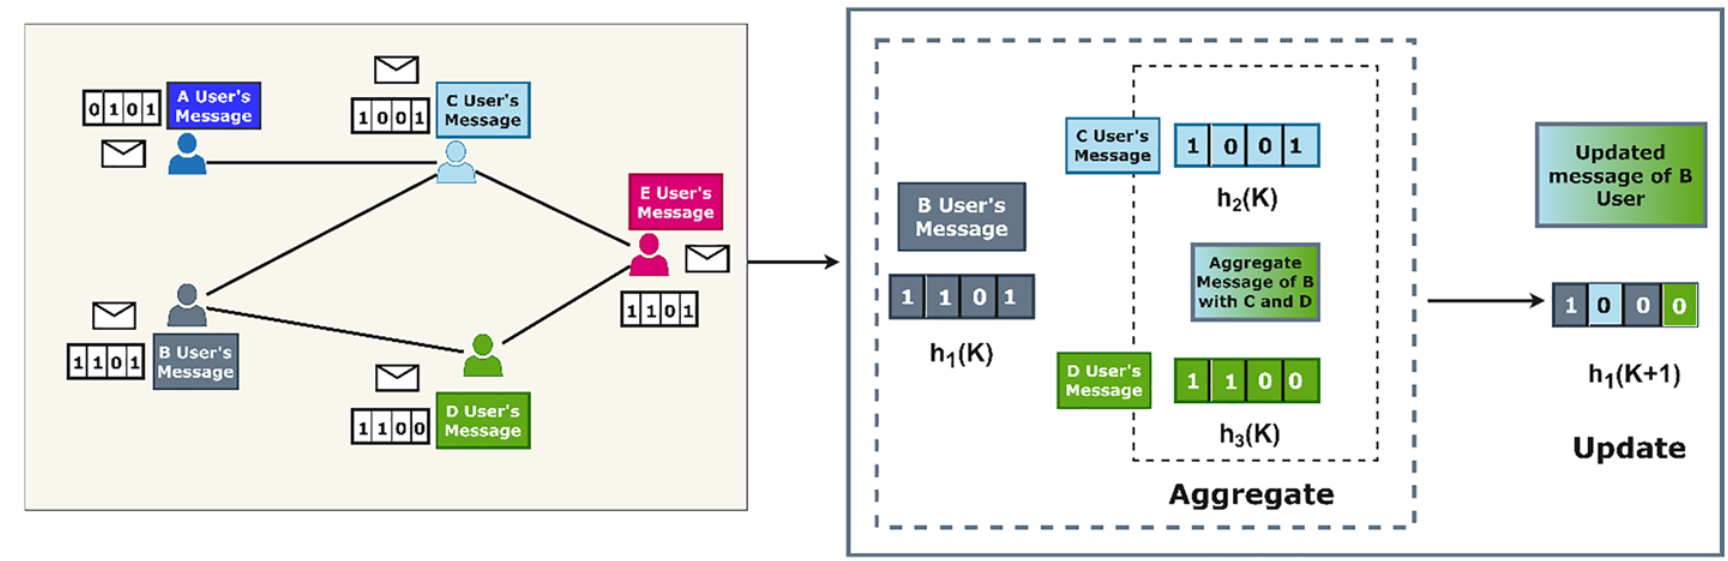
\includegraphics[width=0.9\textwidth]{images/khemani7.png}
\caption{A graphic representation of the update schema for message passing graph neural networks. Taken from \cite[Fig. 7]{khemaniReviewGraphNeural2024}.}
\label{fig:messagepasisng}
\end{figure}



\section{Results}
\label{sec:Results}
In the following, I will give a chronological overview of the topics I worked on during this project. 
This started with the generation of training data, namely Bravais lattices in two and three dimensions. After this, I worked on Bravais lattice classification of noisy and defective lattices to gain familiarity with the GNN architecture and a Machine Learning library. Lastly, I worked on defect detection using Graph Autoencoders. 

\subsection{Generation of training data}
\label{ssec:Generation of training data}
As a first step, Bravais lattices in two dimensions (2D) and three dimensions (3D) needed to be created. 
For this, ideal Bravais lattices with unit spacing between nodes are created in a first step. 
Additionally, random Gaussian noise is added. 
For further variety in training samples, graphs are additionally scaled by random constants to provide non-uniform node spacing within one Bravais lattice group. 
At this step, different kinds of defects are introduced. 
These defects either are the removal of randomly many nodes at random positions or the addition of a single, randomly placed node within the lattice. 
What kind of process has been used will be explained in detail in the following sections, as it is dependent on the task at hand. 
The connections between nodes are then determined by searching for the neighbors within a given radius (that also depends on the noise amplitude) and connecting all nodes, that lie within the said radius. 
By these means the random noise and defects are also included within the structure of the graph and have an influence on message passing. \\

All features used depend on the task of the GNN -- either graph classification into one of the Bravais lattice groups or defect detection. 
In the following, an in-depth overview of all the different features used is given such that the later sections can focus on explaining the Neural Network. \\
As edge features a selection of the following was used: 
\begin{itemize}
\item The 2D or 3D connection vectors between nodes
\item Their respective length
\end{itemize}
The node features tested are the following:
\begin{itemize}
\item The amount of nearest neighbors i.e. the count of connected nodes
\item The bond orientational order parameter (BOO)\\
As the name suggests the BOO quantifies the "order" of the bonds around a node. 
It can be computed for different orders $l$ and can be used to differentiate between different crystal structures by quantifying their $l$-fold symmetry, see e.g. \cite{boo3d}. 
Importantly, symmetry is broken near defects, which is why the BOO seems a promising node feature for defect detection. 
In 2D the BOO of node $j$ and order $l$ is given by \cite{boo2d}
\begin{equation}
\label{eq:boo2d}
\mathrm{BOO^{2D}}_j = \left|\frac{1}{N} \sum_k \mathrm{exp}(il\theta_{jk}) \right|^2
\end{equation}
Where the sum runs over all $N$ neighbors $k$ of node $j$ and $\theta_{jk}$ represents the angle of the $j$-$k$-connection with respect to some fixed reference direction. \\
In 3D, I used one of the rotational invariants defined as \cite{boo3d}
\begin{equation}
\mathrm{BOO^{3D}}_j = \sqrt{\frac{4\pi}{2l+1} \sum_{m=-l}^{l} \left| \frac{1}{N} \sum_k Y_{lm}\right|^2}
\end{equation} 
Here the sum ranges again over all neighbors $k$ and adds the spherical harmonics $Y_{lm}$ dependent on the given order of the BOO and the angles between nodes $j$ and $k$ and an arbitrary reference direction. 
As rotational symmetry is also broken at the edges of the generated graphs, for the calculation of the BOO I take care to apply sufficient padding of extra nodes around the graph (which are later removed) in order to mitigate edge effects. 
\end{itemize}

\subsection{Bravais lattice classification}
\label{ssec:Bravais lattice classification}
The main goal of this chapter is to gain familiarity with a machine learning Python library by working on graph classification of 2- and 3-dimensional Bravais lattices. 
For this, I chose PyTorch, as it has a library for working with graph neural networks called PyTorch Geometric (PyG) built on top of it. 
The first step for both cases was to generate the training data, which was done according to \autoref{ssec:Generation of training data}. 
For this task I chose to add noise to the nodes and remove a random percentage of nodes to introduce some defects. 
The BOO (of orders $l=2,4,6,8,10$) as well as the number of nearest neighbors  were chosen as nodal features. 
Each graph was equipped with a one-hot-encoded label representing the Bravais lattice type it belongs to. 
Additionally, I tested two different layer types, namely GCNConv \cite{pygteamGCNConv2025} and GINEConv layers \cite{pygteamGINEConv2024}. 
I performed both tests as GINEConv layers support edge features in contrast to GCNConv layers and I wanted to gain familiarity with both architectures. 
If edge features were used, I chose for them the length of each edge. 
An example showing how 2D and 3D graphs look like is shown in \autoref{fig:2d 3d lattice}. 

\begin{figure}[htbp]
    \centering
    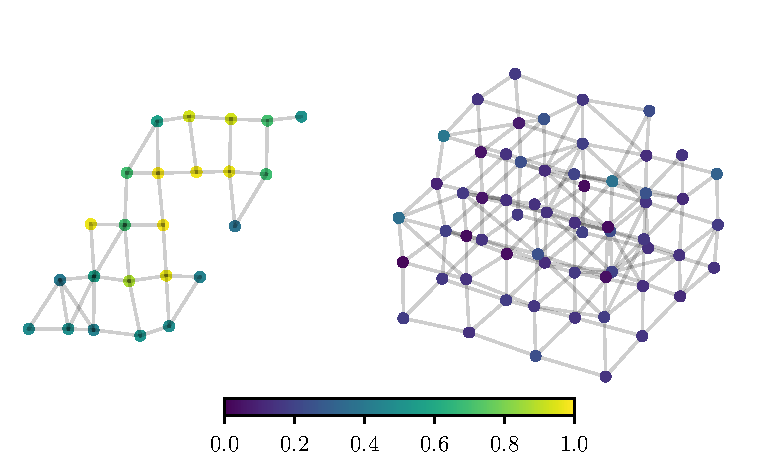
\includegraphics{images/plots/2d_3d_lattice.pdf}
    \caption{On the left an example of an oblique plane graph is shown. The color coded nodes represent the BOO of order $l=2$. Looking at the connectivity of nodes it is clear that noise and defects have a visible influence. The same is true for the orthorhombic primitive 3D lattice shown on the right. Looking at the node features it becomes apparent that the BOO in 3 dimensions seems to be less variable than in 2D. This is visible for all orders, although here only the second order is shown.}
    \label{fig:2d 3d lattice}
\end{figure}

For the 2D case both networks consisted of three layers, the input of dimensionality 6 is expanded in the first hidden layer to a feature dimensionality of 8, then reduced in dimensionality to 6 again in the second hidden layer. 
Both hidden layers were followed by $\mathrm{tanh}$ as a non-linear activation function. 
After these hidden layers classification layers were introduced. 
For this a dimensionality reduction from $N * 6$ (with $N$ the number of nodes) to 5 (the number of classes) is needed. 
This is achieved by using a global mean pooling layer to reduce the dimensions from $N * 6$ to $6$ followed by a dense linear layer to reduce them further from $6$ to $5$. 
For completeness, it should be noted, that in the following a batch size of 16 is used, which is why all dimension stated above are in reality higher by a factor of 16. 
This was left out in the above discussion to make the layer construction more clear. \\
Cross Entropy was used as a loss function and for the optimizer I chose Adam with a learning rate $\eta=0.005$. 
Evaluation of the model was then done by calculating the fraction of correct classifications over a test dataset that was not used during training. 
For this the networks output is interpreted as an unnormalized probability of each class being the correct one. 
For testing, it is then checked whether the network assigns the highest probability to the correct label or not. 
250 graphs per lattice type with a size of 5 times 5 nodes were created, as this has proven itself to be sufficient for classification in 2D. 
1000 graphs were used for training 5 times 50 epochs (meaning the training of 50 epochs was repeated 5 times and averaged to be less dependent on random network initialization) and 250 graphs were used for validation. 
The results of training are shown in \autoref{fig:bravais classification 2d}. 
\begin{figure}[htbp]
    \centering
    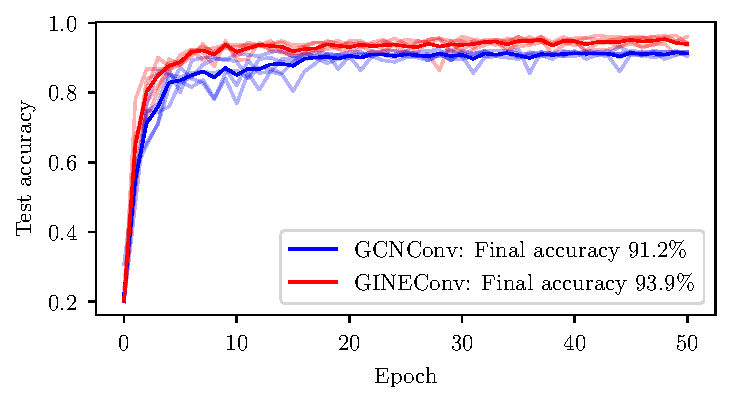
\includegraphics{images/plots/2d_classifier_results.pdf}
    \caption{The resulting test accuracy for the different network architectures is shown. For this five random initializations were run (translucent curves) and then averaged (dark curves). It is apparent that GINEConv layers work better. }
    \label{fig:bravais classification 2d}
\end{figure}
It is clearly visible that GINEConv layers perform better than GCNConv layers. 
This makes sense as the GINEConv network has additional information, namely the edge lengths as edge features. 
A final averaged accuracy of $93.9\%$ has been reached, 2D Bravais lattice classification can therefore be deemed successful. \\

In 3D the same features, network layers, loss and other hyperparameters were chosen with the only difference being the increased amount of hidden layers (3 instead of 2) and their feature dimensionality. 
This increase is needed to reach good performance as 3D graphs are more complex than 2D ones. 
Here the dimensionality increases from 6 to 10 to 20 to 30 in the three hidden layers (which are also followed by $\mathrm{tanh}$ as non-linear activation) and reach the required dimension of 14 by use of a global mean pooling and linear layer for classification. 
Again 250 graphs (of size 5 times 5 times 5 nodes) were generated for each class of which 3000 were used for training and the remaining 500 for testing. 
All other things remain exactly the same as with the 2D case. 
The training results are shown in \autoref{fig:bravais classifacation 3d}. 
\begin{figure}[htbp]
    \centering
    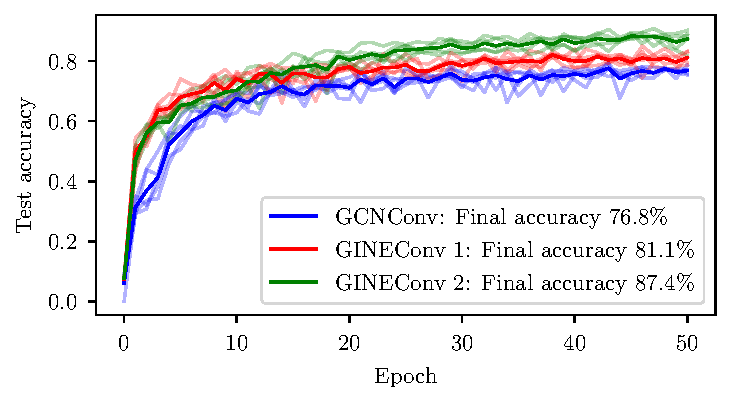
\includegraphics{images/plots/3d_classifier_results.pdf}
    \caption{The training results of the 3D Bravais lattice classification are shown. GCNConv and GINEConv 1 tests were performed with the BOO and the number of neighbors as node attributes. Furthermore, a test with the same features as chosen at the time of the intermediate report is shown as GINEConv 2. As edge features the 3D connection vectors (not lengths) were chosen and for node attributes only the number of neighbors was used. It is visible that this configuration performs best.}
    \label{fig:bravais classifacation 3d}
\end{figure}
Again, the best results were achieved by using GINEConv layers due to priorly mentioned reasons. 
However, as the test accuracy was not quite satisfactory ($81.1\%$) I performed additionally a test with the graph features that I chose at the time of the intermediate report, corresponding to the green curve in \autoref{fig:bravais classifacation 3d}. 
For this the edge features were chosen to be the connection vectors instead of their length, and the node features were reduced to only encompassing the number of neighbors. 
Other than that, the network setup and training remained exactly the same. 
This achieved a much better accuracy of $87.4\%$ indicating that the BOO in 3D is less meaningful than in 2D at least when it comes to lattice classification. 
This fits to the less variable BOO in 3D observed in \autoref{fig:2d 3d lattice}. 
In summary, when not using the BOO the network still performs rather well, especially considering that in 3D there exist 14 classes instead of only 5 and the false positive rate (the network by chance guesses the correct class) is expected to be much lower. 
Therefore, also 3D Bravais lattice classification can be deemed successful. 

\subsection{Defect detection}
\label{ssec:Defect detection}
\subsubsection{Introduction}
The next goal was to build a GNN tasked with defect detection in 2D and 3D lattices utilizing the Dominant network \cite{dingDeepAnomalyDetection2019}. 
As this has proven itself to be quite hard, the following chapters will give an overview of the tests I performed and their evaluation rather than straight-forwardly presenting a positive result. 
For this, the general setup and network architecture is explained in a first step, after which all different tests will be explained and analyzed. 
At the end, I will discuss possible reasons for the bad performance of the Dominant network.
Lastly, in \autoref{sec:Conclusion} I will draw a conclusion of the networks performance and suggest approaches that may be better suited for defect detection. 
It should be noted that I will focus the following discussion on noise-free 2D graphs, firstly because of time constraints due to the extensive tests I needed to do, and secondly, because it is not helpful or illustrative to investigate noisy or more complex and worse visualizable 3D graphs when even the simplest 2D cases show bad performance. \\

Data was generated as described in \autoref{ssec:Generation of training data}. 
As I investigated different feature combinations, the exact features used will be shown for each test specifically. 
Features were taken out of the feature pool shown in \autoref{ssec:Generation of training data}. 
Per graph, one defect was added by adding a node at a random position. 
This defect node is different from the others both on a structural level, because it has higher connectivity than the rest of the graph, but also on an attribute level. 
This is because it breaks symmetry which has an influence on the BOO, additionally, on average, the length of connected edges is smaller and the number of neighbors higher. 
As mentioned noise was not added for the following tests to make it even easier for the network to detect the outlier node. 
In \autoref{fig:features_2d_lattices} a few lattices are shown together with their feature space to illustrate how the features differ between the anomalous node and the more regular ones. \\

\begin{figure}[htbp]
    \centering
    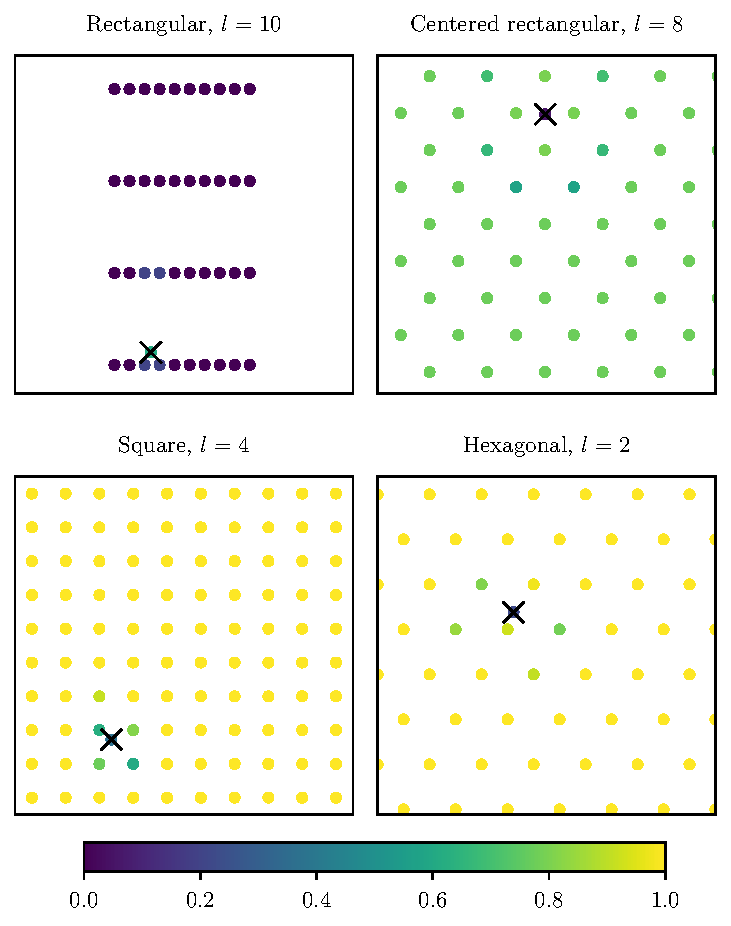
\includegraphics{images/plots/features_2d_lattices.pdf}
    \caption{Shown is the feature space of 4 of the 5 Bravais lattices introduced in \autoref{ssec:Bravais lattices}. It is visible how the BOO of different orders $l$ highlights the additional node in each case. Some lattices were zoomed in for better visibility. The anomalous node is marked by a black cross.}
    \label{fig:features_2d_lattices}
\end{figure}

I looked at many different network setups, layers, and features and therefore needed to keep the training time in a reasonable scope which is why I chose to use 250 graphs for each of the 5 Bravais lattice types. 
This resulted in a total of 1250 graphs, of which 1000 were used for training and 250 for validation. 
Each network/feature combination test consisted of training the network over 50 epochs and averaging the results over five different random network initializations in order to achieve good convergence of the loss curves and a statistically more meaningful result. 
For all the following tests, a batch size of 16 and the Adam optimizer were used. 
If the test used edge features GINEConv layers \cite{pygteamGINEConv2024} were used for the construction of the encoder and attribute decoder, else GCNConv layers \cite{pygteamGCNConv2025} were used.
As the learning rate, activation functions, and the number of neurons and layers were varied, they will be stated explicitly when talking about the specific test performed. \\

\subsubsection{The Dominant Architecture}
I was tasked to implement the Dominant network as described in \cite{dingDeepAnomalyDetection2019}. 
This network uses a graph autoencoder i.e. an autoencoder consisting of message passing layers to handle graphs. 
Autoencoders are a special kind of neural network that utilize unsupervised training. 
The goal of this type of network is to reconstruct the input data as best as possible. 
This task would be trivial if it were not for an important feature of autoencoders: 
The hidden layers reduce in dimensionality until a minimum number of trainable parameters is reached at the so-called bottleneck after which the dimensionality again increases until the input dimensionality. 
It is expected that this compression and decompression works better for large-scale recurring structures (e.g. a periodic arrangement of nodes) than for outliers (e.g. the defect node) which makes this approach promising for the task at hand \cite{dingDeepAnomalyDetection2019}. 
A sketch of the structure of the Dominant network is shown in \autoref{fig:Dominant}.
\begin{figure}[htbp]
\centering
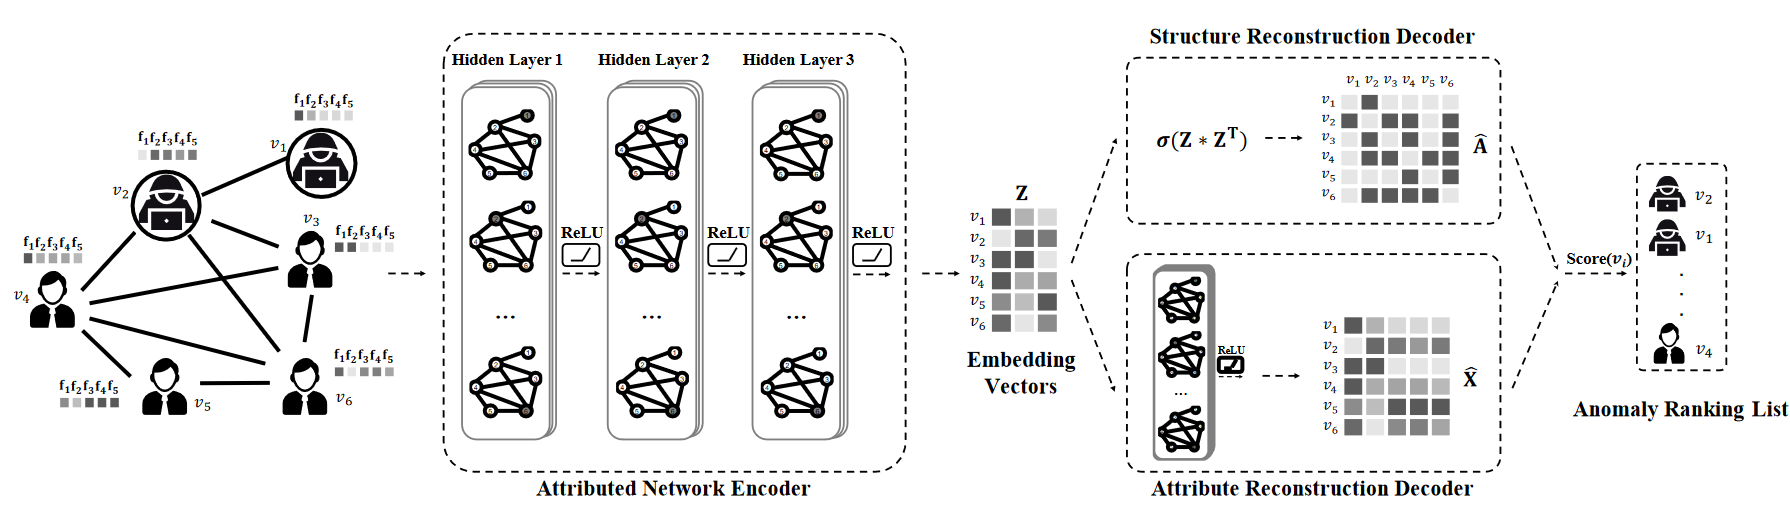
\includegraphics[width=\textwidth]{images/ding_1.png}
\caption{A sketch of the structure of the Dominant network is shown. The shown number of layers and activation functions do not necessarily reflect the ones used in the following, as different tests have been performed. Taken from \cite[Fig.1]{dingDeepAnomalyDetection2019}}
\label{fig:Dominant}
\end{figure}
A training set of graphs with outliers is first input into the encoder, this is represented by the graph on the left of \autoref{fig:Dominant}. 
This attributed network encoder consists of message-passing layers that reduce in feature dimensionality until the bottleneck is reached. 
The graph data is maximally compressed into so-called embedding vectors $z$, which can be interpreted as a matrix. 
This is then decoded in two different decoders (see \autoref{fig:Dominant}): 
The structure reconstruction decoder aims to reproduce the input adjacency matrix, which is a possible representation of the edges and their features in a graph. 
This is done by calculating the matrix product of the matrix $z$ with the matrix $z^T$ leading to a matrix of shape $N\cross N$ where $N$ is the number of nodes. 
The product can then be interpreted as an adjacency matrix. 
Furthermore, a non-linear activation function (like a sigmoid) can be applied. 
Additionally, the attribute reconstruction decoder aims to reproduce the nodal features of the input graph. 
This is done by the use of an additional GNN which increases in feature dimensionality. 
In the following, I choose the encoder and decoder network symmetrically. 
After getting both reconstructions a loss can be calculated (this is not shown in \autoref{fig:Dominant}) with which the model is trained \cite{dingDeepAnomalyDetection2019}:
\begin{equation}
\label{eq:dominant loss}
\mathcal{L} = (1-\alpha) \left\lVert A-\hat{A} \right\rVert _F + \alpha \left\lVert X-\hat{X} \right\rVert _F
\end{equation}
Here $\alpha$ is a fixed hyperparameter weighting the attribute versus the reconstruction loss, $A$ and $\hat{A}$ are the input and reconstructed adjacency matrices, $X$ and $\hat{X}$ the input and reconstructed node feature matrices and the symbol $\left\lVert\cdot \right\rVert _F$ represents the Frobenius norm. 
Note that compared to \cite{dingDeepAnomalyDetection2019} I have omitted squaring the norms as this would have led to extremely large losses which would have needed additional normalization to achieve a good convergence without offering any benefit. 

Once training is deemed sufficient, a final anomaly score can be calculated for each node $i$ to evaluate the model \cite{dingDeepAnomalyDetection2019}:
\begin{equation}
\label{eq:dominant score}
\mathcal{S}_i = (1-\alpha) \left\lVert a_i-\hat{a_i} \right\rVert _2 + \alpha \left\lVert x_i-\hat{x_i} \right\rVert _2
\end{equation}
Here $\alpha$ is the loss weight of \autoref{eq:dominant loss}, $a_i$, $\hat{a}_i$, $x_i$, $\hat{x}_i$ represent the rows of the matrices $A$, $\hat{A}$, $X$, $\hat{X}$ respectively and $\left\lVert\cdot \right\rVert _2$ represents the usual vector 2-norm. 
Note that while \autoref{eq:dominant loss} and \autoref{eq:dominant score} look rather similar, they are not quite the same. 
The loss function computes a single scalar loss for each input graph and is used during training. 
The anomaly score function computes one scalar anomaly score for each node in the graph and is only used for evaluation. 
Larger anomaly scores represent a higher probability of the node being an outlier. \\

When evaluating the model's anomaly score in practice the result is a 1D vector consisting of "unnormalized probabilities" for every graph where each entry corresponds to the anomaly score of the node at the given index. 
In principle, these values could be normalized to a value range of 0-1 such that they could be interpreted as the probability of the given node being an outlier. 
This is however not done as it is not necessary for the further steps. 
Instead, all anomaly score vectors of the evaluation dataset are combined into a single metric (called score in the following) quantifying the performance of the network. 
This score is given by the average probability of the true anomalous node being in the top five anomaly scores the network predicts. 
The top 5 anomaly scores are checked, as all input features are different from the background not only at the additional node but also at the nodes surrounding it (see also \autoref{fig:features_2d_lattices}). 
Because of this also a guess in the neighborhood of the additional node should be considered correct which is why it also increases the score. 
Note that because correspondence with the true position of the additional node (i.e. the graph label) is checked in the score evaluation, using the score during training would be a supervised learning approach and defeat the purpose of the autoencoder. 
Therefore, I want to emphasize again, that the training is done in an unsupervised manner (using the loss) and the score only represents an evaluation metric. 


\subsubsection{Results}
I performed multiple tests with differently structured layers, activation functions, learning rates $\eta$, loss weights $\alpha$, dropout, and data parameters. 
These I will present in the following to show, that no matter the chosen hyperparameters the training and performance of the NN is bad. 
In the first step, $\eta$ and the use of dropout was varied, after which the best features, network structure, activation functions, and $\alpha$ were explored in subsequent tests. 
When varying one or two related parameters the others were kept fixed. 
All hyperparameters for the different tests A-E are tabularised in \autoref{tab:hyperparameters defect detection} for referencing them in \autoref{fig:defect detection A} - \autoref{fig:defect detection E}. 

\begin{table}[htbp]
\centering
\begin{tabular}{c|c|c|c|c|c|c|c|c|c}
test & layers & structure & A-act. & S-act. & $\eta$ & DO & $\alpha$ & NN & BOO \\\hline\hline
A1 & GINE & 6432 & $\sigma$ & ReLu & 0.001 & \no & 0.5 & \yes & \yes \\\hline
A2 & - & - & - & - & 0.005  & -  & - & - & - \\\hline
A3 & - & - & - & - & 0.01   & -  & - & - & - \\\hline
A4 & - & - & - & - & 0.0005 & \yes & - & - & - \\\hline
A5 & - & - & - & - & \cellcolor{black!20} 0.001  & \cellcolor{black!20} \yes & - & - & - \\\hline
A6 & - & - & - & - & 0.003  & - & - & - & - \\\hline
A7 & - & - & - & - & 0.005  & - & - & - & - \\\hline
A8 & - & - & - & - & 0.01   & - & - & - & - \\\hline\hline
B1 & GINE & 6432 & $\sigma$ & ReLu & 0.001 & \yes & 0.5 & \cellcolor{black!20}\yes & \cellcolor{black!20}\yes \\\hline
B2 & - & - & - & - & - & - & - & \no & \yes \\\hline
B3 & - & - & - & - & - & - & - & \no & $l\neq2$ \\\hline\hline
C1 & GCN & 6432  & ReLu & ReLu & 0.001 & \yes & 0.5 & \yes & \yes \\\hline
C2 & - & 6543  & -   & -   & -   & -   & -  & -   & -   \\\hline
C3 & \cellcolor{black!20}GCN &\cellcolor{black!20} 6531  & -   & -   & -   & -   & -  & -   & -   \\\hline
C4 & - & 65432 & -   & -   & -   & -   & -  & -   & -   \\\hline
C5 & GINE& 6432  &$\sigma$& ReLu & 0.001 & \yes & 0.5 & \yes & \yes \\\hline
C6 & -& 6543  & -   & -   & -   & -   & -  & -   & -   \\\hline
C7 & -& 6531  & -   & -   & -   & -   & -  & -   & -   \\\hline
C8 & -& 65432 & -   & -   & -   & -   & -  & -   & -   \\\hline\hline
D1 & GCN & 6432 &$\sigma$&$\sigma$& 0.001 & \yes & 0.5 & \yes & \yes \\\hline
D2 & -  & -   &$\sigma$& none  & -   & -   & -  & -   & -   \\\hline
D3 & -  & -   &\cellcolor{black!20}  ReLu  & \cellcolor{black!20} ReLu  & -   & -   & -  & -   & -   \\\hline
D4 & -  & -   & ReLu  & none  & -   & -   & -  & -   & -   \\\hline
D5 & -  & -   & ReLu  &$\sigma$& -   & -   & -  & -   & -   \\\hline\hline
E1 & GCN & 6432 & ReLu & ReLu & 0.001 & \yes & 0.3 & \yes & \yes \\\hline
E2 & -  & -   & -   & -   & -   & -  &\cellcolor{black!20} 0.4 & -  & -    \\\hline
E3 & -  & -   & -   & -   & -   & -  & 0.5 & -  & -    \\\hline
E4 & -  & -   & -   & -   & -   & -  & 0.6 & -  & -    \\\hline
E5 & -  & -   & -   & -   & -   & -  & 0.7 & -  & -    \\\hline\hline
\end{tabular}
\caption{Listed are the used hyperparameters for each test A-E. Each row corresponds to one network/data combination that was used for training 5 times 50 epochs which were then averaged to produce the curves in \autoref{fig:defect detection A} - \autoref{fig:defect detection E}. "-" means the parameter is the same as in the row above. Cells with a gray background indicate the best results of each test. The columns represent from left to right: The used layer (either GINEConv or GCNConv), the dimensionality of the encoder layers with mirrored decoder (e.g. 6432 means the input node feature vector of dimension 6 is reduced to a hidden feature vector of dimension 4 in the first, 3 in the second hidden layer and 2 in the bottleneck), the attribute (A-act.) and structure (S-act.) decoder activation functions, the learning rate, whether a dropout (DO) with probability 0.5 was used, the loss weighting, whether the number of nearest neighbors (NN) or the bond orientational order parameter (BOO) have been used as features.}
\label{tab:hyperparameters defect detection}
\end{table}

As mentioned in the first test the influence of the learning rate $\eta$ and the use of dropout were examined. 
To make matters easier a dropout with a fixed probability of 0.5 has been applied between each layer during training. 
For evaluation, this dropout is automatically switched off. 
For this first test, it seemed best to supply the network with maximal information, which is why all node features (BOO of order $l=2,4,6,8,10$ and the number of neighbors) were used as well as the length of edges as edge features. 
Because edge features are used, GINEConv layers are employed in a structure of 6432, meaning the input feature vector dimensionality is reduced from 6 to 4 to 3 to 2 in the encoder and increased again symmetrically in the attribute decoder. 
As activation a sigmoid was used after each hidden layer for the attribute reconstruction taking care not to apply a sigmoid to the output. 
A ReLu function was used for the structure decoder, as the adjacency matrix can have values bigger than 1 depending on the edge features. 
All these choices are also listed in \autoref{tab:hyperparameters defect detection} and will therefore be discussed less extensively for the following tests. \\
Now the network was run for larger and smaller $\eta$ in combination with dropout or without dropout for 5 times 50 epochs. 
For each training epoch, the network was evaluated by calculating its loss and detection score based on a test sample that was not used during training.
These curves are then averaged over the mentioned 5 random network initializations to get a more robust and comparable result, as single runs have proven themselves to be very dependent on initialization. 
The results are shown in \autoref{fig:defect detection A}, where one can see that the network performs best if dropout and $\eta=0.001$ are implemented (labelled A5 in \autoref{fig:defect detection A}). 

\begin{figure}[htbp]
\centering
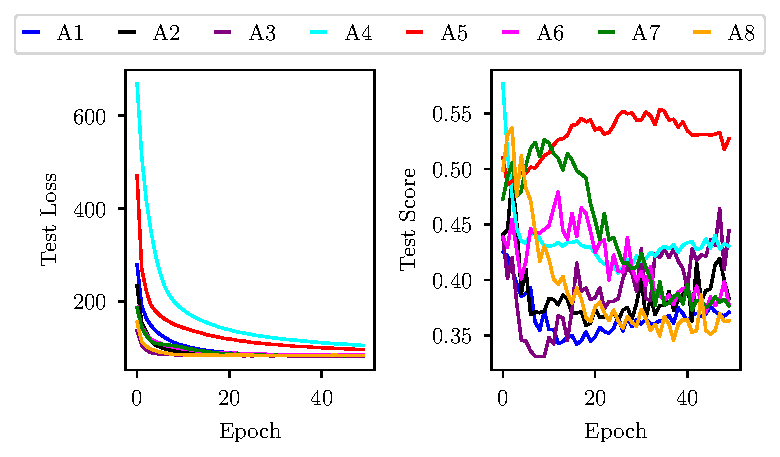
\includegraphics{images/plots/defect_detection_A.pdf}
\caption{Shown are the test results for Test A. Each curve is the average result of 5 random network initializations. For a listing of hyperparameters see \autoref{tab:hyperparameters defect detection}.}
\label{fig:defect detection A}
\end{figure}

However, the central problem that will also govern the tests shown in the following becomes apparent. 
While the loss is minimized quite well by the network and a stable loss is reached after around 50 epochs indicating the network has trained all it can given the input network and data parameters, the score behaves quite differently. 
Namely, there are two problems. 
Firstly, it is immediately apparent that the score does not increase steadily with falling loss. 
Rather it increases and decreases seemingly at random even for the "optimal" parameter choice shown in red. 
Looking at all curves a slight downward trend is even visible. 
Secondly one can see the score already starts on quite a high level of roughly 50\% correct guesses. 
However, as the score is determined by the percentage of test graphs where the true anomalous node is within the top five highest anomaly scores and there are roughly 100 nodes in each graph the initial score should be much lower if the network would just perform a random guess. 
This indicates the network in its untrained state is in fact not performing random guesses but rather there is a systematic component "pushing" the network towards the right guess even when all weights are initialized randomly. 
I reason this follows from the nature of how the anomalous node affects the graph and the network structure. 
A spurious node increases connectivity around it as it increases local density and with that the amount of connected nodes as they are determined by connecting all nodes within a said radius. 
In the message passing layers this highly connected node now receives more messages that are additionally different from those other more regular nodes receive. 
The number of neighbors for instance is higher on average, while the edge length is lower and the BOO also differs in all orders. 
I assume that this increases the mean squared reconstruction error of this node on average even for a random initialization and therefore leads to a slightly higher anomaly score in a local neighborhood around the anomalous node. 
This in turn leads to the fact that the network has quite good performance from the start. \\
What I want to stress however is that this high score should not be interpreted as a success in achieving the given task. 
This is because it is not a learned behavior but rather just stems from systematics that indicates that a machine learning approach with this architecture is not well suited for defect detection as learning is de facto not needed. 
This might further indicate that there could be a simpler algorithm that does not use Machine Learning but can extract the anomalous node just from the connectivity and feature space of the graph itself. \\

This general result is also visible in the next four tests I performed. 
In the next step, I wanted to establish what kind of node features are useful for the network. 
The result of this is shown in \autoref{fig:defect detection B}. 
\begin{figure}[htbp]
\centering
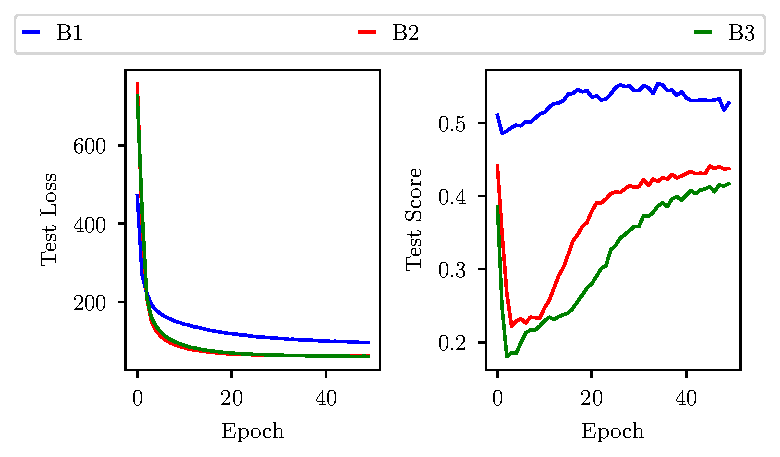
\includegraphics{images/plots/defect_detection_B.pdf}
\caption{Shown are the test results for Test B. Each curve is the average result of 5 random network initializations. For a listing of hyperparameters see \autoref{tab:hyperparameters defect detection}.}
\label{fig:defect detection B}
\end{figure}
The motivation behind this test was mainly to see whether the number of neighbors was a good node feature or not and how many degrees of the BOO are useful for the network. 
I expected the neighbor-information to be already present in the general connectivity of the graph to some extent and therefore wanted to quantify the difference between using this feature and not using it.  
The result is that the network performs best when given the maximal amount of information, i.e. the BOO of order $l=2,4,6,8,10$ and the number of neighbors are used (this test is labelled B1). 
However, it should again be stated that the evaluation metric that interests us in the end, namely the score, has the same behavior as before, leading to the same conclusion that the network is not learning to do the desired task of outlier detection. \\

As test C I performed a variation of the network layers, the number of layers, and feature dimensionality in them. 
The switch in layers also meant a switch in features as only the GINEConv layers support edge features, meaning none were used for the GCNConv layers. 
The result is shown in \autoref{fig:defect detection C}. 

\begin{figure}[htbp]
\centering
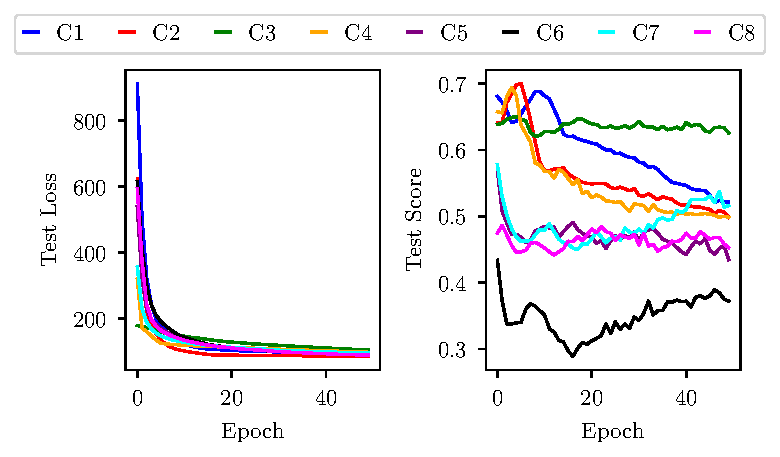
\includegraphics{images/plots/defect_detection_C.pdf}
\caption{Shown are the test results for Test C. Each curve is the average result of 5 random network initializations. For a listing of hyperparameters see \autoref{tab:hyperparameters defect detection}.}
\label{fig:defect detection C}
\end{figure}

As one can see in the graphic the network seemingly works best if no edge features are present and GCNConv layers are used instead. 
I don't expect the reason for this to be that the network works better with less information however (especially as the edge length usually pinpoints quite well where the additional node is present). 
Looking at the starting score of the different curves in \autoref{fig:defect detection C} it becomes apparent that it is already much higher for the GCNConv layers than for the GINEConv layers. 
During training, both then fluctuate seemingly at random again and partly increase or decrease. 
The better performance of one layer over the other can therefore be attributed to the same systematic effect that leads to the high score in the beginning for all layer types and is not due to the model being better at classification. 
Nevertheless, the tests I performed indicated the best performance with GCNConv layers of the structure 6531 (test C3). \\

The test shown in \autoref{fig:defect detection D} now focused on the question which activation function to use. 
\begin{figure}[htbp]
\centering
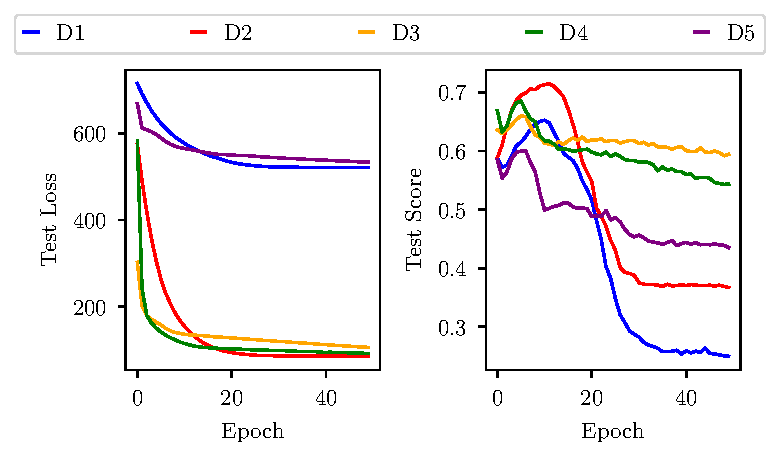
\includegraphics{images/plots/defect_detection_D.pdf}
\caption{Shown are the test results for Test D. Each curve is the average result of 5 random network initializations. For a listing of hyperparameters see \autoref{tab:hyperparameters defect detection}.}
\label{fig:defect detection D}
\end{figure}
I expected a sigmoid to perform badly as attribute activation as there are nodal attributes that are larger than unity which would be truncated leading to a big reconstruction error. 
This is indeed what the test D1, D2 and D5 show as well. 
The best combination has proven itself to be ReLu as both activations (D3). 
However, again the previously mentioned issues with the score curves are visible. \\


As a last test, I varied the $\alpha$ parameter. 
Looking at the calculation of the loss and score function in \autoref{eq:dominant loss} and \autoref{eq:dominant score} it becomes clear that $\alpha$ varies the weight of structure reconstruction loss over the attribute reconstruction loss and score. 
The test curves shown in \autoref{fig:defect detection E} indicate the best performance for $\alpha=0.4$ (E2) as it performs only slightly worse than $\alpha=0.3$ (E1) but seems to be more stable. \\

\begin{figure}[htbp]
\centering
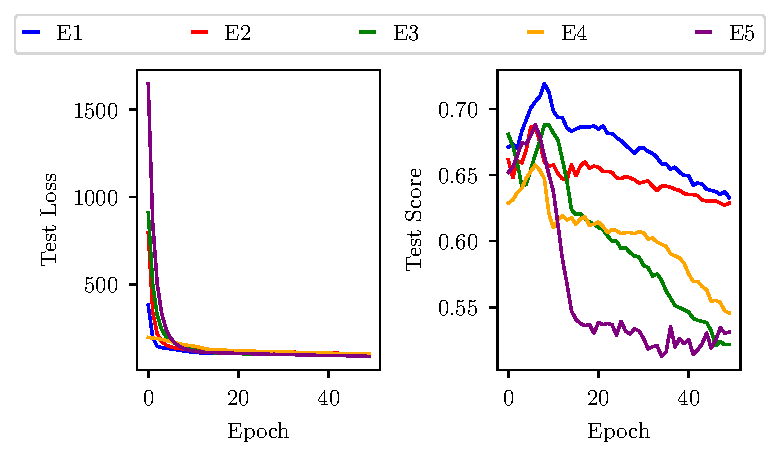
\includegraphics{images/plots/defect_detection_E.pdf}
\caption{Shown are the test results for Test E. Each curve is the average result of 5 random network initializations. For a listing of hyperparameters see \autoref{tab:hyperparameters defect detection}.}
\label{fig:defect detection E}
\end{figure}

In summary, all tests shown above indicate bad performance of the model in the task of learning to classify defects in 2D lattices. 
Even though the resulting scores are quite high (at times well above 60\%) they are not high because the model has learned to classify lattices through the use of the graph autoencoder but rather because there is a systematic component in the structure of the graph data and the GNN itself leading to very high scores from the beginning. 
These high scores then only fluctuate and mostly even decay while training, all while the training objective function (the loss) gets smaller and smaller. 
In other words: 
The model is not bad at the task it trains for. 
During training the loss function is minimized well by use of gradient descent and backpropagation techniques introduced in \autoref{ssec:BAsics of Machine Learning}. 
Therefore, it succeeds in reproducing the \emph{features} of nodes and edges well. 
However, this does not translate to the model getting better at \emph{identifying outliers} which is the task we want it to perform in the end. \\
With the extensive amount of tests that were performed, I further showed that this is not simply due to a bad choice of hyperparameters or data features but rather a very fundamental problem with the architecture itself. 
It should further be emphasized again that this result was achieved with the simplest Bravais lattices one can think of. 
Planar graphs without any noise, boundary effects, or other special cases like missing nodes have been considered to make learning to identify outliers easy. 
Additionally, features have been chosen to give a large amount of information, essentially each feature points directly to the spurious node in the graph (see \autoref{fig:features_2d_lattices}). 
That learning still does not work therefore again indicates that the Dominant-architecture is not well suited for the task at hand.

\section{Conclusion}
\label{sec:Conclusion}
In \autoref{ssec:Bravais lattice classification} I worked on Bravais lattice classification of 2D and 3D lattices. 
For this I generated noisy lattices according to the 5 (or 14 in 3D) Bravais groups, introduced defects and labelled them by using one hot encoding. 
In the 2D case I performed tests with GCNConv and GINEConv graph convolutional layers and achieved maximum training prediction accuracies of roughly $94\%$ by using comparably small graphs consisting of roughly 25 nodes and a shallow network with only two hidden layers. 
In 3D, I was able to reach an accuracy of roughly $87\%$ by using graphs consisting of around 125 nodes and a network with 3 hidden layers. 
I showed how the BOO in 3D is less suited for the lattice classification than that in 2D. 
Both results can probably be improved even further by having a more detailed investigation regarding hyperparameters and network structure. 
This was however not the focus of this work.
Instead, the results shown here make clear that lattice classification is a task well suited for a GNN and can be seen as a motivation for a further project that deepens the analysis performed here. \\

In \autoref{ssec:Defect detection} I then went on to perform defect detection on graphs using the Dominant architecture proposed in \cite{dingDeepAnomalyDetection2019}. 
For this I generated noiseless plane graphs and introduced a single spurious, labelled node that the network should identify. 
I have shown that even for this simplified, 2D noiseless case the performance of a Dominant-type network is bad. 
While the loss function is minimized rather well, this does not translate to the score of correctly classified defects that interests us in the end. 
I performed extensive tests of different network architectures, hyperparameters and features to show that the observed bad performance is independent of them. 
Training of the network in defect detection does not seem to happen, instead the score is dominated by systematics that stem from the GNN and the way messages are passed itself. 
Due to time constraints the exact systematic effect mentioned could not be determined or quantified. 
This could be an interesting study for future projects. 
Additionally, it would be interesting to compare the performance of the Dominant architecture to models that work differently, e.g. by using node prediction directly instead of using an autoencoder. 
Node prediction with one hot encoded node labels, i.e. the use of supervised learning, seem a promising alternative as the issue of having separate loss and score functions could be mitigated. 
I could imagine that solving this separation a rising score could be linked more closely to a falling loss (which is as mentioned before not really the case with the Dominant network). \\

In summary the work presented here shows that GNNs are in principle well suited for work with crystal lattices. The positive and especially negative results shown motivate further projects in lattice classification and defect detection and lay the groundwork for these by discussing approaches for lattice generation, feature choice and network architecture.


\section{Code availability}
\label{sec:Code availability}
The code written for this project is made available in the following Git repository: \url{https://github.com/SteWey0/Computerpraktikum/}

%---------------------------------------------------------
%   Bibliography
%---------------------------------------------------------

% \newgeometry{
%     %a4paper,
%     left=40mm,
%     % right=20mm,
%     top=35mm,
% }
\renewcommand\refname{Bibliography}
% \printbibliography
\printbibliography[
heading=bibintoc,
title={Bibliography}
]


\end{document}